\chapter{Extremal Moment Problems}
\label{Ch: MomentProblems}

\lhead{Chapter \ref{Ch: MomentProblems}. \emph{Extremal Moment Problems}} % This is for the header on each page
\definecolor{niceblue}{rgb}{0,0.1,0.5}
%----------------------------------------------------------------------------------------
%	Chapter Text
%----------------------------------------------------------------------------------------

%\section*{Introduction}
For $k = 0,1,\dots,n$ we are given a sequence of continuous and linearly independent functions, $u_k: [a,b] \mapsto \mathbb{R}$, and a sequence of moments, $c_k \in \mathbb{R}$. A moment problem asks for which distributions, $\sigma$, (if any) the moments can be represented as
\begin{align}
c_k &= \int_a^b u_k(t) \intd \sigma(t) && k = 0,1,\dots,n
\label{eq:momentproblem}
\end{align}
where either $a$ or $b$ or both may be infinite. We call \eqref{eq:momentproblem} a \emph{representation} of the moment sequence. A typical extremal problem is that, given a continuous function $\Omega(t)$, find
\begin{equation}
\min_\sigma \left( \int_a^b \Omega(t) \intd \sigma(t)\right)
\end{equation}
where $\sigma$ satisfies \eqref{eq:momentproblem} for given $u_k$ and $c_k$.

For now we will focus on the problem with $a$ and $b$ finite. Most of the basic results transfer easily to the case in which either $a$ or $b$ or both are infinite \cite{Krein1977-ak}. 

\section{Geometrical Interpretation}
Much of the following theory can be more easily understood from a geometrical viewpoint. Instead of thinking of our $u_k$ and $c_k$ as series, we can write
\begin{equation}
\vect{u}(t) = (u_0(t),u_1(t),\dots,u_n(t))
\end{equation}
and
\begin{equation}
\vect{c} = (c_0,c_1,\dots,c_n)
\end{equation}
where $\vect{u}: [a,b] \mapsto \mathbb{R}^{n+1}$ and $\vect{c} \in \mathbb{R}^{n+1}$.

\subsection{Convex Conical Hulls}
Of importance to our geometrical understanding of the moment problem are conic and convex sets and convex conical hulls. A set $C$ is \emph{conic} (Figure \ref{fig:conicset}) if for all $t \geq 0$, $\vect{x} \in U$ implies $t\vect{x} \in C$. A set $C$ is \emph{convex} (Figure \ref{fig:convexset}) if for all $t \in [0,1]$, $\vect{x}_1,\vect{x}_2 \in C$ implies $t\vect{x}_1 + (1-t)\vect{x}_2 \in C$.
\begin{figure}[ht]
	\centering
	\begin{minipage}[b]{0.45\linewidth}
		\centering
		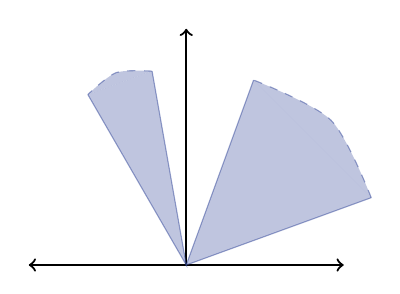
\begin{tikzpicture}
			\coordinate (A1) at (20:2.5);
			\coordinate (A-curve) at (45:2.6);
			\coordinate (A2) at (70:2.5);
			\coordinate (B1) at (100:2.5);
			\coordinate (B-curve) at (110:2.6);
			\coordinate (B2) at (120:2.5);
			%Axis
			\draw[thick,<->] (-2,0) -- (2,0);
			\draw[thick,->] (0,0) -- (0,3);
			%Conical Set
			\path[fill=niceblue!50, draw=niceblue!80, opacity = 0.5] (A1) -- (0,0) --  (A2);
			\path[fill=niceblue!50, draw=niceblue!80, opacity = 0.5] (B1) -- (0,0) --  (B2);
			\path[dashed,fill=niceblue!50,draw=niceblue!80,opacity = 0.5] plot [smooth] coordinates {(A1) (A-curve) (A2)};
			\path[dashed,fill=niceblue!50,draw=niceblue!80,opacity = 0.5] plot [smooth] coordinates {(B1) (B-curve) (B2)};
		\end{tikzpicture}
		\subcaption{}\label{fig:conicset}
	\end{minipage}
	\begin{minipage}[b]{0.45\linewidth}
		\centering
		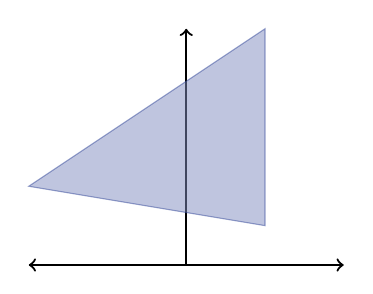
\begin{tikzpicture}
			%Axis
			\draw[thick,<->] (-2,0) -- (2,0);
			\draw[thick,->] (0,0) -- (0,3);
			%Convex set
			\path[fill=niceblue!50, draw=niceblue!80, opacity = 0.5] (-2,1)--(1,0.5)--(1,3)--cycle;
		\end{tikzpicture}
		\subcaption{}\label{fig:convexset}
	\end{minipage}
	\caption{A set which is conic but not convex (\subref{fig:conicset}) and a set which is convex but not conic (\subref{fig:convexset}). The dashed curves symbolize that the regions extend infinitely.}
\end{figure}

The \emph{convex conical hull} of a set $U$ is the intersection of all convex conical sets that contain $U$. Similarly, the \emph{closed convex conical hull} of a set $U$ (Figure \ref{fig:closedconicalhullofU}) is the intersection of all closed convex conical sets that contain $U$. We denote the closed convex conical hull of $U$ with $\coni(U)$.
\begin{figure}[ht]
	\centering
	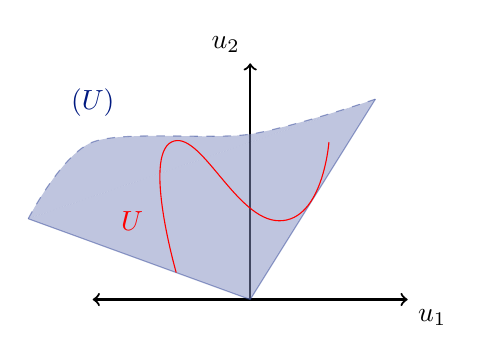
\begin{tikzpicture}
		\coordinate (O) at (0,0);
		\coordinate (A) at (160:1);
		\coordinate (B) at (-1,2);
		\coordinate (C) at (0.37,1);
		\coordinate (D) at (1,2);
		%Axis
		\draw[thick,<->] (-2,0) -- (2,0) node[anchor=north west] {$u_1$};
		\draw[thick,->] (0,0) -- (0,3) node[anchor=south east]{$u_2$};
		%Conical Hull
		\path[fill=niceblue!50, draw=niceblue!80, opacity = 0.5] (58:3) -- (O) --  (160:3);
		\path[dashed,fill=niceblue!50, draw=niceblue!80,opacity = 0.5] plot [smooth] coordinates {(160:3) (-2,2) (0,2.1) (58:3)};
		%Curve U
		\draw[red] plot [smooth, tension=1] coordinates {(A) (B) (C) (D)};
		%Labels
		\draw (-1.5,1) node {$\color{red}{U}$};
		\draw (-2,2.5) node {$\color{niceblue}{\coni(U)}$};
	\end{tikzpicture}
	\caption{The closed convex conical hull (blue) of the curve $U$ (red). The dashed curve symbolizes that the region extends infinitely.}\label{fig:closedconicalhullofU}
\end{figure}

The following is a fundamental theorem on conical hulls \cite{Krein1977-ak}.
\begin{theorem}
	Let $U = \left \lbrace \vect{u}(t) : a \leq t \leq b \right\rbrace$ be a curve. Then $\coni(U)$ is the set of points $\vect{c}$ that satisfy
	\begin{equation}
		\vect{c} = \int_a^b \vect{u}(t) \intd \sigma(t)
	\end{equation}
	for some mass distribution $\sigma$.
	\label{thm:conicalhulls}
\end{theorem}


\subsection{Convex Hulls}
The \emph{convex hull} of a set $U$ is the intersection of all convex sets that contain $U$. The \emph{closed convex hull} of a set $U$ (Figure \ref{fig:closedconvexhullofU}) is the intersection of all closed convex sets that contain $U$. We denote the closed convex hull of $U$ with $\conv(U)$.
\begin{figure}[ht]
	\centering
	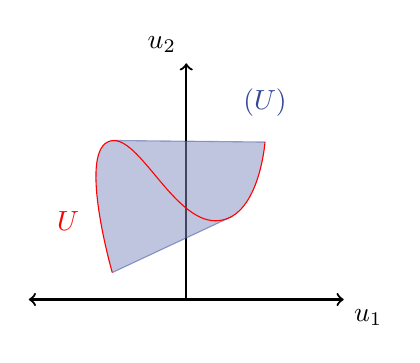
\begin{tikzpicture}
		\coordinate (O) at (0,0);
		\coordinate (A) at (160:1);
		\coordinate (B) at (-1,2);
		\coordinate (C) at (0.37,1);
		\coordinate (D) at (1,2);
		%Hacky nasty guess work
		\coordinate (blah1) at (0.58,1.054);
		\coordinate (blah2) at (-0.93,2.02);
		\coordinate(blahmid) at (0,1.145);
		%Axis
		\draw[thick,<->] (-2,0) -- (2,0) node[anchor=north west] {$\color{black}{u_1}$};
		\draw[thick,->] (0,0) -- (0,3) node[anchor=south east]{$\color{black}{u_2}$};
		%Convex Hull
		\path[fill = niceblue!50, opacity = 0.5] 
		plot [smooth, tension=1] coordinates{(A) (B) (C) (D)}
		(A) -- (blah1)--(blahmid)--cycle
		(D) --  (blahmid) -- (blah2) -- cycle;
		\path[draw = niceblue!80, opacity  = 0.5]
		(A) -- (blah1)
		(D) -- (blah2);
		%Curve U
		\draw[red] plot [smooth, tension=1] coordinates {(A) (B) (C) (D)};
		%Labels
		\draw (-1.5,1) node {$\color{red}{U}$};
		\draw (1,2.5) node {$\color{niceblue!80}{\conv(U)}$};
	\end{tikzpicture}
	\caption{The closed convex hull (blue) of the curve $U$ (red).}\label{fig:closedconvexhullofU}
\end{figure}

A slight variation on Theorem \ref{thm:conicalhulls} is the following \cite{Krein1977-ak}.

\begin{theorem}
	Let $U = \left \lbrace \vect{u}(t) : a \leq t \leq b \right\rbrace$ be a curve. Then $\conv(U)$ is the set of points $\vect{c}$ that satisfy
	\begin{equation}
	\vect{c} = \int_a^b \vect{u}(t) \intd \sigma(t)
	\end{equation}
	for some probability distribution $\sigma$.
	\label{thm:convexhulls}
\end{theorem}

Note that we can ensure $\sigma$ is a probability distribution by requiring that it satisfy
\begin{equation}
	\int_a^b \intd \sigma(t) = 1.
\end{equation}

%\subsection{Application back to problem bit}
%Theorems \ref{thm:conicalhulls} and \ref{thm:convexhulls}
\subsection{Positive Sequences}
Given our sequence of continuous and linearly independent function $u_k$, we can define polynomials, $P: [a,b] \mapsto \mathbb{R}$, of the form
\begin{equation}
	P(t) = \sum_{k = 0}^n \alpha_k u_k(t).
\end{equation}
We create a functional, $\PolyFunc$, on these polynomials
\begin{equation}
	\PolyFunc \left(P(t)\right) = \PolyFunc \left(\sum_{k = 0}^n \alpha_k u_k(t)\right) = \sum_{k=0}^n \alpha_k c_k
\end{equation}
where the $c_k$ are our given moment sequence. 

We say that our moment sequence is \emph{positive} (relative to the $u_k$) if for all non-negative $P(t)$ we have that $\PolyFunc(P) \geq 0$. This becomes \emph{strictly positive} if $\PolyFunc(P) > 0$ for all such $P$ and singularly positive if there exists a non-negative $P_0 \not\equiv 0$ such that $\PolyFunc(P_0) = 0$.
\begin{theorem}
	A moment sequence, $\vect{c} = (c_0,c_1,\dots,c_n)$, is strictly (singularly) positive with respect to $\vect{u}(t) = (u_0(t),u_1(t),\dots,u_n(t))$ if and only if it is an interior point (boundary point) of $\coni(U)$ (where $U = \left\{ \vect{u}(t): a\leq t\leq b\right\}$).
\end{theorem}

\section{Canonical Representations}
We are particularly interested in the case where \eqref{eq:momentproblem} involves a discrete distribution $\sigma$ with finitely many point masses. If $\sigma$ has points masses $\rho_1, \rho_2, \dots, \rho_m$ at locations $t_1 < t_2 <\dots < t_m$ ($a \leq t_1, t_m \leq b$) then \eqref{eq:momentproblem} becomes
\begin{align}
	c_k &= \sum_{j=1}^m \rho_j u_k(t_j) && k = 0,1,\dots,n.
\end{align}
We define the index of the above representation to be
\begin{equation}
	\sum_{j = 1}^m \epsilon(t_j)
\end{equation}
where $\epsilon(t) = 2$ for $a < t<b$ and $\epsilon(a) = \epsilon(b) = 1$. A representation is \emph{canonical} if its index is less than or equal to $n+2$ and \emph{principal} if its index is less than or equal to $n+1$. A principal representation is \emph{upper} if $t_m = b$ and \emph{lower} otherwise.

\begin{theorem}[Probably only true for Chebyshev systems... maybe move sections around]
	If the $c_k$ are strictly positive then they have exactly one lower principal representation and one upper principal representation.
	\label{thm: Unique LPR and UPR}
\end{theorem}
\begin{proof}
	IDEA: Every point in conical hull can be written as conical combination of $n+1$ points
	Caratheodory show that you can definitely find principal representations. Not so clear how to show that there are only two. Actually doesn't... dimensions don't match up. Plus that's irrelevant as we're talking about INDEX...
	
	What does this theorem imply about conical hulls? Convex hulls?
\end{proof}

REMARK: N odd and even different types

\section{Chebyshev Systems}
The functions $u_k(t): S \mapsto \mathbb{R}$ ($k = 0,1,\dots,n$) form a \emph{Chebyshev system ($T$-system)} if any non-trivial polynomial of these functions,
\begin{align}
P(t) &= \sum_{k=0}^n \alpha_k u_k(t) &&\alpha_k \in \mathbb{R}
\label{eq: Chebyshev Polynomial}
\end{align}
has no more than $n$ zeros (on $S$). This is equivalent to requiring that the determinant
\begin{equation}
\left| \begin{tabular}{cccc}
$u_0(t_0)$ & $u_1(t_0)$ &\dots & $u_n(t_0)$\\
$u_0(t_1)$ & $u_1(t_1)$ &\dots & $u_n(t_1)$\\
\vdots & \vdots & $\ddots$ & \vdots\\
$u_0(t_n)$ & $u_1(t_n)$ &\dots & $u_n(t_n)$
\end{tabular}\right|
\label{eq: Chebyshev Determinant}
\end{equation}
is not zero for any choice of $t_0 < t_1 < \dots < t_n \in S$. The functions $u_k$ form a \emph{Chebyshev plus system ($T_+$-system)} if the determinant in \eqref{eq: Chebyshev Determinant} is always positive. We say that $u_{n+1}$ is a \emph{$T$-extension ($T_+$-extension)} of a $T$-system ($T_+$-system) $\{u_k(t)\}_0^n$ if $\{u_k(t)\}_0^{n+1}$ is also a $T$-system ($T_+$-system).

We will only consider functions defined on intervals, $S = [a,b]$. A zero, $t_0$, of the polynomial in \eqref{eq: Chebyshev Polynomial} is classified as \emph{nodal} if $P(t)$ changes sign around $t_0$ and \emph{non-nodal} if it does not (zeros at $a$ or $b$ will be considered \emph{nodal}).


%Geometrical interpretation on page 34


\section{Extremal Theory}
\begin{theorem}
	If the $u_k$ form a $T_+$-system on $[a,b]$, and $\Omega$ is a $T_+$-extension of this system, the minimum (maximum) value of 
	\begin{equation}
	\int_a^b \Omega (t) \intd \sigma(t)
	\end{equation}
	where $\sigma$ must satisfy
	\begin{align}
	\int_a^b u_k(t) \intd \sigma(t) &= c_k && k = 0,1,\dots,n
	\label{eq: Moment Constraints (thm Extremal Value)}
	\end{align}
	is obtained for the lower (upper) principal distribution.
	\label{thm: Extremal values of an integral}
\end{theorem}

The proof of this theorem requires the following lemma.
\begin{lemma}
	\label{lem: Non-negative Polynomial with m non-nondal zeros}
	Given a $T_+$-system ($u_k(t)$, $k = 0,\dots,n$), on $[a,b]$ of order $n = 2m $, and $m$ points $t_1,\dots,t_m \in (a,b)$, we can construct a non-negative polynomial with non-nodal zeros at the given $m$ points and no other zeros.
\end{lemma}
\begin{proof}
	Let $\beta$ denote the set of polynomials of the form in \eqref{eq: Chebyshev Polynomial}. Let $\beta_B \subset \beta$ be the set of polynomials such that $\sum_{k=0}^{n} \alpha_k^2 = 1$.
	%beta_B for bounded
	COMPACT BLAH
	
	Choose sequences $t_1^l, t_2^l,\dots,t_m^l$ such that $t_1 < t_1^l<\dots<t_m<t_m^l<b$ and
	$$\lim_{l \rightarrow \infty} t_j^l = t_j.$$
	We define
	\begin{equation}
	P_l(t) = C_l \left|
	\begin{tabular}{cccc}
	$u_0(t)$ & $u_1(t)$&\dots & $u_{2m}(t)$\\
	$u_0(t_1)$ & $u_1(t_1)$&\dots & $u_{2m}(t_1)$\\
	$u_0(t_1^l)$ & $u_1(t_1^l)$&\dots & $u_{2m}(t_1^l)$\\
	\vdots & \vdots & $\ddots$ & \vdots\\
	$u_0(t_m)$ & $u_1(t_m)$&\dots & $u_{2m}(t_m)$\\
	$u_0(t_m^l)$ & $u_1(t_m^l)$&\dots & $u_{2m}(t_m^l)$
	\end{tabular}
	\right|
	\label{eq: P_l determinant}
	\end{equation}
	where $C_l$ is the positive scaling factor such that $P_l(t) \in \beta_B$. Clearly, $P_l(t)$ has zeros at $t = t_1,t_1^l,\dots,t_m,t_m^l$. Since the $u_k$ form a $T_+$-system, $P_l(t)$ must be positive for $t \in [a,t_1)$. For $t \in (t_1,t_1^l)$, $P_l(t)$ must be negative (since if we switched rows 1 and 2 of \eqref{eq: P_l determinant} we would get something positive MAKE BETTER). Continuing this argument we find that
	\begin{align}
	P_l(t) &> 0 \text{ for } t \in [a,t_1) \cup (t_1^l,t_2) \cup \dots \cup (t_{m-1}^l,t_m) \cup (t_m,b]\\
	\label{eq: P_l(t) > 0}
	P_l(t) &< 0 \text{ for } t \in (t_1,t_1^l) \cup (t_2,t_2^l) \cup \dots \cup (t_{m},t_m^l).
	\end{align}
	
	Since $\beta_B$ is compact, $P_l$ converges to some $P_\infty \in \beta_B$. $P_\infty$ is non-negative by \eqref{eq: P_l(t) > 0} and has clearly has zeros only at $t_1,t_2,\dots,t_m$. Finally, these zeros must be non-nodal as $P_\infty(t)$ is non-negative.
\end{proof}

\begin{proof}[Proof of Theorem \ref{thm: Extremal values of an integral} ]
	This is for my own benefit. 
	We start with the case $n = 2m -1$.	In this case, the lower principal distribution, $\sigma(t)$, has $m$ masses interior to $[a,b]$. %Reference back?
	We want to construct a non-negative polynomial of the form
	\begin{equation}
	P(t) = \sum_{k = 0}^{n+1} \alpha_k u_k(t)
	\end{equation}
	that has a non-nodal zero at the location of each mass in $\sigma$. Here, $u_{n+1}(t) = \Omega(t)$ (since $\Omega$ is a $T_+$-extension of our $T_+$-system this notation is justified). One such polynomial is $P_\infty(t)$, as defined in Lemma \ref{lem: Non-negative Polynomial with m non-nondal zeros}. Now consider the integral
	\begin{equation}
	\int_a^b P_\infty(t) \intd \sigma_L(t)% = \alpha_{k+1} \int_a^b \Omega(t) \sigma_L(t) + \int_a^b \left(\sum_{k=0}^n \alpha_k u_L(t)\right) \intd \sigma_L(t)
	\end{equation}
	where $\sigma_L(t)$ is the lower principal distribution.
	Since $P_\infty$ is zero precisely at the masses of $\sigma_L$,
	\begin{equation}
	\int_a^b P_\infty(t) \intd \sigma_L(t) = 0.
	\end{equation}
	Now let $\sigma \neq \sigma_L$ be any other distribution that satisfies \eqref{eq: Moment Constraints (thm Extremal Value)}. Theorem \ref{thm: Unique LPR and UPR}, along with the non-negativity of $P_\infty$, imply that
	\begin{equation}
	\int_a^b P_\infty(t) \intd \sigma(t) > 0.
	\end{equation}
	From \eqref{eq: Moment Constraints (thm Extremal Value)} we get
	\begin{equation}
	 \int_a^b P_\infty(t) \intd \sigma(t) = \alpha_{k+1} \int_a^b \Omega(t) \sigma(t) + \sum_{k=0}^n \alpha_k c_k
	 \end{equation}
	 and so
	 \begin{equation}
	 \alpha_{k+1} \int_a^b \Omega(t) \sigma_L(t) + \sum_{k=0}^n \alpha_k c_k < \alpha_{k+1} \int_a^b \Omega(t) \sigma(t) + \sum_{k=0}^n \alpha_k c_k
	 \end{equation}
	 which implies
	 \begin{equation}
		 \alpha_{k+1} \int_a^b \Omega(t) \sigma_L(t) <  \alpha_{k+1} \int_a^b \Omega(t) \sigma(t).
		 \label{eq: Final Inequality Alpha}
	 \end{equation}
	 All that is left is to prove that $\alpha_{k+1} > 0$. From \eqref{eq: P_l determinant},
	 \begin{equation}
	 	\alpha_{k+1}^l = (-1)^{2m}C_l\left|
	 	\begin{tabular}{cccc}
	 	$u_0(t_1)$ & $u_1(t_1)$&\dots & $u_{2m-1}(t_1)$\\
	 	$u_0(t_1^l)$ & $u_1(t_1^l)$&\dots & $u_{2m-1}(t_1^l)$\\
	 	\vdots & \vdots & $\ddots$ & \vdots\\
	 	$u_0(t_m)$ & $u_1(t_m)$&\dots & $u_{2m-1}(t_m)$\\
	 	$u_0(t_m^l)$ & $u_1(t_m^l)$&\dots & $u_{2m-1}(t_m^l)$
	 	\end{tabular}\right|.
	 \end{equation}
	 Since the $u_k$ form a $T_+$-system, the above determinant must be non-negative and since $C_l > 0$, $\alpha_{k+1} \geq 0$. We cannot have $\alpha_{k+1} = 0$ as then \eqref{eq: Final Inequality Alpha} wouldn't hold and so $\alpha_{k+1} > 0$. We conclude that
	 \begin{equation}
	 \int_a^b \Omega(t) \sigma_L(t) <  \int_a^b \Omega(t) \sigma(t).
	 \label{eq: Final Inequality}
	 \end{equation}
	 
	
\end{proof}


